\subsection{Desarrollo}
Durante la etapa de desarrollo se realizó la implementación de módulos de lógica musical, el generador de combinaciones, el algoritmo de poda y ramificación y la comprobación del algoritmo a través de pruebas unitarias y una sencilla interfaz gráfica.

\textbf{En primer lugar}, con respecto a los módulos musicales, se comenzó por la implementación de la lógica detras de las \textbf{notas} y \textbf{acordes}:

\begin{itemize}
    \item \textbf{Notas}:
    \begin{itemize}
        \item Interfaz \textit{Note}, con propiedad nombre (latín y anglosajón), \gls{altura tonal} y \gls{octava}.
        \item Objeto \textit{Notes}, mapa de \textit{Note} que representan cada una de las 12 notas.
        \item Métodos para la creación de \textit{Note}, a través de varios parametros o una ristra.
        \item Métodos para la búsqueda de una nota en \textit{Notes} por altura tonal y por nombre.
        \item Métodos para la \gls{transposición} de notas, con funciones para el avance o el retroceso en uno o varios pasos.
    \end{itemize}

    \item \textbf{Acordes}:
    \begin{itemize}
        \item Interfaz \textit{Quality}, con propiedades para la definición de varios nombres \textit{(i.e. para cualidad Mayor se establecen mayor, maj y M)} y conjunto de alturas tonales con pesos.
        \item Objeto \textit{Qualities}, mapa de \textit{Quality} que representan las \gls{cualidad}es mas comunes \textit{(i.e. Mayor, Menor, Disminuida, Aumentada, Septima, Mayor Septima...)}.
        \item Interfaz \textit{Chord}, con propiedad \textit{Note} y \textit{Quality}.
        \item Métodos para la creación de \textit{Chord}, a través de varios parametros o una ristra.
        \item Método de búsqueda de una cualidad en \textit{Qualities} por nombre.
        \item Método de cálculo de cualidad para una nota raíz.
        \item Métodos para la trasposición de acordes, con funciones para el avance o el retroceso en un solo paso.
    \end{itemize}
\end{itemize}

Seguidamente, se desarrolló la lógica correspondiente a los \textbf{instrumentos} y \textbf{diagramas de acordes}:

\begin{itemize}
    \item \textbf{Instrumento}: definición de la interfaz \textit{Instrument}, implementación de función para la creación de instrumentos a partir de los argumentos nombre, número de trastes y cuerdas al aire, representadas como vector de objetos \textit{Nota} o vector de ristras y transposición del instrumento a partir de un número de pasos.

    \item \textbf{Diagrama de Acorde}: definición de la interfaz \textit{ChordDiagram} y creación de diagramas de acordes a partir de los argumentos \textit{Instrument}, \textit{Chord} y profundidad de traste.
\end{itemize}

Los módulos anteriores fueron indispensables para el desarrollo del algoritmo, ya que definen la estructura y lógica musical \textit{(i.e. notas y acordes)} y la relación entre los distintos módulos que satisfacen los requisitos del incremento \figref{fig:modulos_it2}.

\begin{figure}[H]
    \centering
    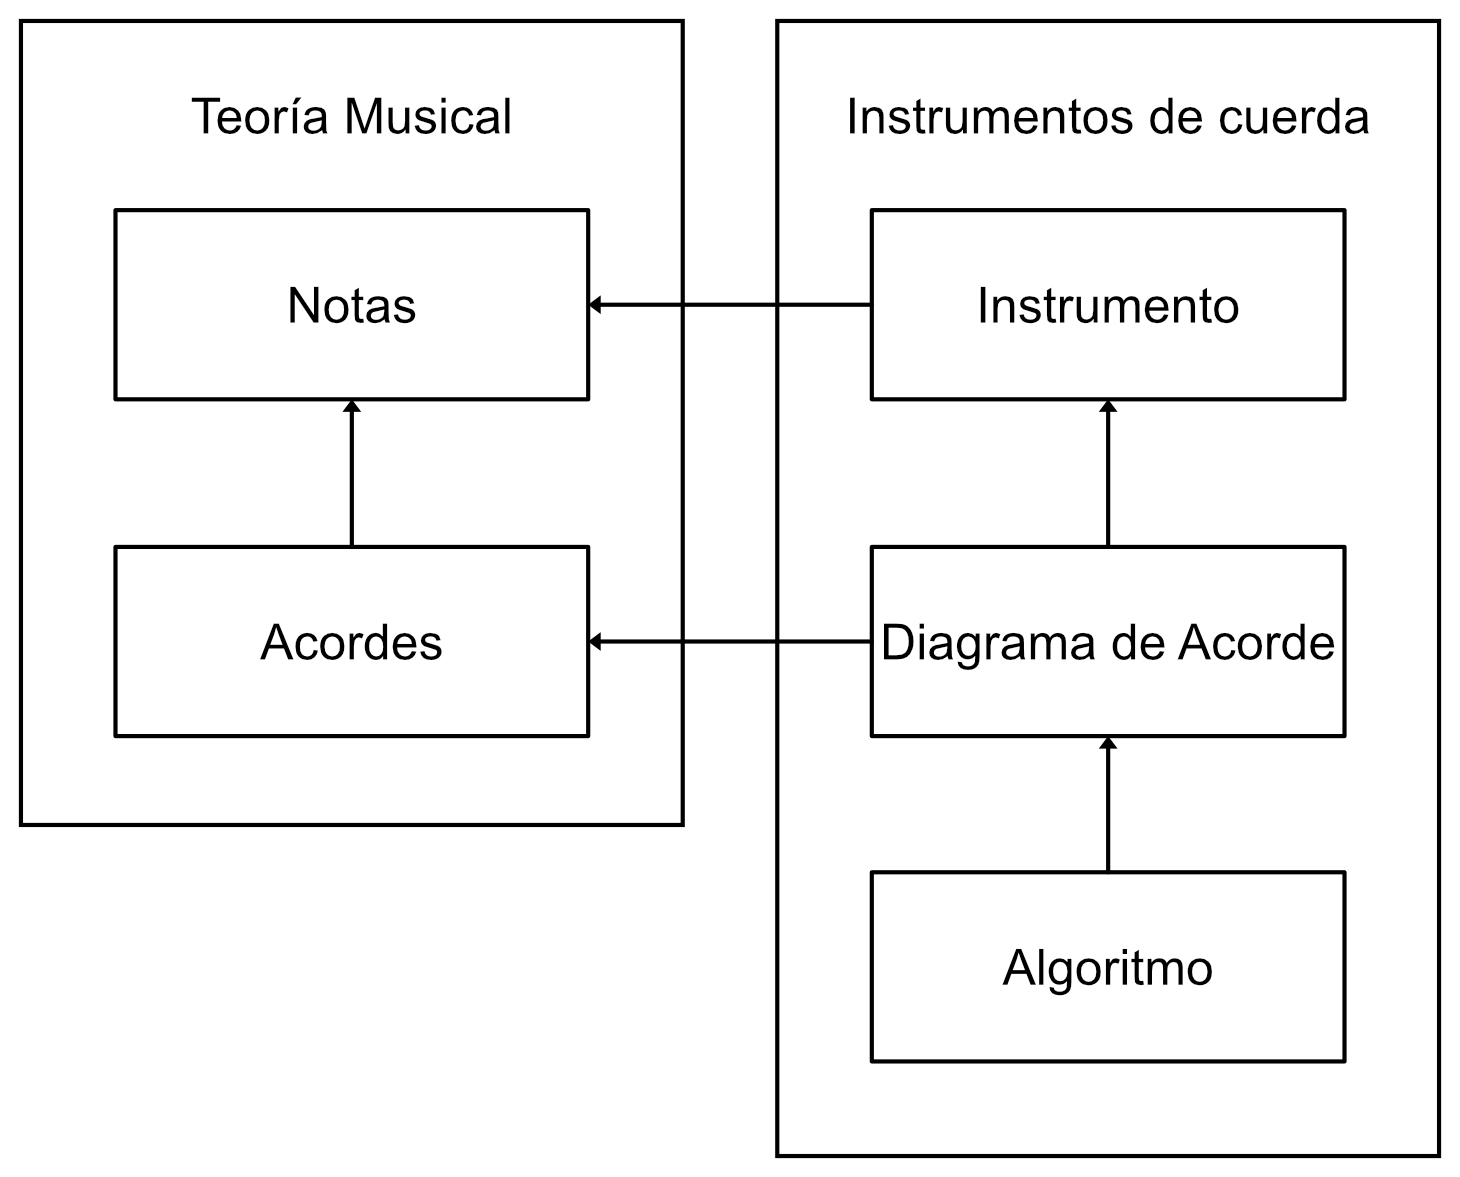
\includegraphics[width=0.5\textwidth]{Ilustraciones/desarrollo/incremento2/desarrollo/modulos_it2.jpg}
    \caption{Organización de módulo del incremento 2}\label{fig:modulos_it2}
\end{figure}

\textbf{En segundo lugar}, se implementó un método para la generación de combinaciones \algoref{a:combinaciones} que explorá los trastes del instrumento en busca de notas que coincidan con las que conforman el acorde.

\begin{algorithm}[H]
\begin{algorithmic}
\scriptsize
\Function{CalcularCombinaciones}{acorde, instrumento, profundidad}
    \State combinaciones $\gets$ lista vacía
    \ForAll{notaAlAire \textbf{en} instrumentoTransportado}
        \State trastesPosibles $\gets$ lista vacía
        \For{traste = 0 \textbf{a} profundidad}
            \State notaEnTraste $\gets$ \textsc{transponerNota}(notaAlAire, traste)
            \If{notaEnTraste está en acorde}
                \State apilar traste en trastesPosibles
            \EndIf
        \EndFor
        \If{trastesPosibles no está vacío}
            \State apilar trastesPosibles en resultado
        \Else
            \State apilar [-1] en combinaciones
        \EndIf
    \EndFor
    \State \Return combinaciones
\EndFunction
\end{algorithmic}
\caption{Cálculo de posiciones posibles de trastes para un acorde}\label{a:combinaciones}
\end{algorithm}

\textbf{En tercer lugar}, se desarrolló el algoritmo de ramificación y poda \algoref{a:podayrama}, y las funciones para la evaluación de variantes parciales o completas. Para ello, se utilizó una  aproximación de búsqueda en profundidad recursiva:

\begin{enumerate}
    \item Un bucle \textit{for-each} para la exploración de la segunda dimensión del vector combinaciones.
    \item Recursion para la exploración de la primera dimensión del vector combinaciones.
\end{enumerate}

De este modo, se construyen variantes seleccionando un valor de la segunda dimensión para cada elemento de la primera \textit{(i.e. un traste para cada cuerda)}. El algoritmo retrocede recursivamente para explorar las diferentes combinaciones posibles. Se establece la poda al inicio de cada iteración:

\begin{enumerate}
    \item Se evalúan los dedos disponibles.
    \item Se evalua la facilidad de reproducción de la variante parcial.
    \item Si la variante es completa, se evalua su correctitud musical. Esta puntuación se suma a la facilidad de reproducción y se compara la puntuación total con la de la mejor variante encontrada hasta el momento.
\end{enumerate}

\begin{algorithm}[H]
\caption{calculateChordFretPositions}\label{a:podayrama}
\scriptsize
\begin{algorithmic}
\Procedure{CalcularPosicionesAcorde}{$indiceCuerda,$
            $combinaciones,$
            $resultado,$
            $dedos,$
            $cejilla,$
            $notasAlAire,$
            $acordeRaiz,$
            $mejorVariante$}

    \If{$dedos > 4$}
        \State \Return
    \EndIf

    \State $varianteParcial \gets \{dedos, cejilla, resultado, puntuacion\}$
    \State $puntuacionParcial \gets$ EvaluarTocabilidad($varianteParcial$)

    \If{$puntuacionParcial \geq mejorVariante.puntuacion$}
        \State \Return
    \EndIf

    \If{$indiceCuerda = combinaciones.tamano$}
        \State $puntuacionFinal \gets puntuacionParcial$ + EvaluarCorrectitudMusical($varianteParcial, notasAlAire, acordeRaiz$)

        \If{$puntuacionFinal < mejorVariante.puntuacion$}
            \State $mejorVariante \gets varianteParcial$
        \EndIf

        \State \Return
    \EndIf

    \ForAll{$traste$ \textbf{en} $combinaciones[indiceCuerda]$}
        \If{$trasteEnCejilla$}
        \ElsIf{$esCuerdaAlAire$}
            \State $cejillaActual \gets traste$
            \State $dedoActual \gets indiceCuerda$
        \ElsIf{$trasteBajoCejilla \land trastePresionado$}
            \State $cejillaActual \gets traste$
            \State $dedoActual \gets indiceCuerda + 1$
        \ElsIf{$hayDedosDisponibles \land trastePresionado$}
            \State $dedoActual \gets dedoActual + 1$
        \EndIf

        \State apilar traste en resultado

        \State \Call{CalcularPosicionesAcorde}{
            $indiceCuerda + 1,$
            $combinaciones,$
            $resultado,$
            $dedoActual,$
            $cejillaActual,$
            $notasAlAire,$
            $acordeRaiz,$
            $mejorVariante$
        }

        \State desapilar en resultado

    \EndFor

\EndProcedure
\end{algorithmic}
\end{algorithm}

\textbf{Finalmente}, comprobó la efectividad del algoritmo de dos formas. Por un lado, se realizaron pruebas unitarias \figref{fig:test_it2} para todos los módulos implementados, comenzando por notas y acordes, siguiendo diagramas de acordes y instrumentos, y finalizando con el algoritmo de acordes.

\begin{figure}[H]
    \centering
    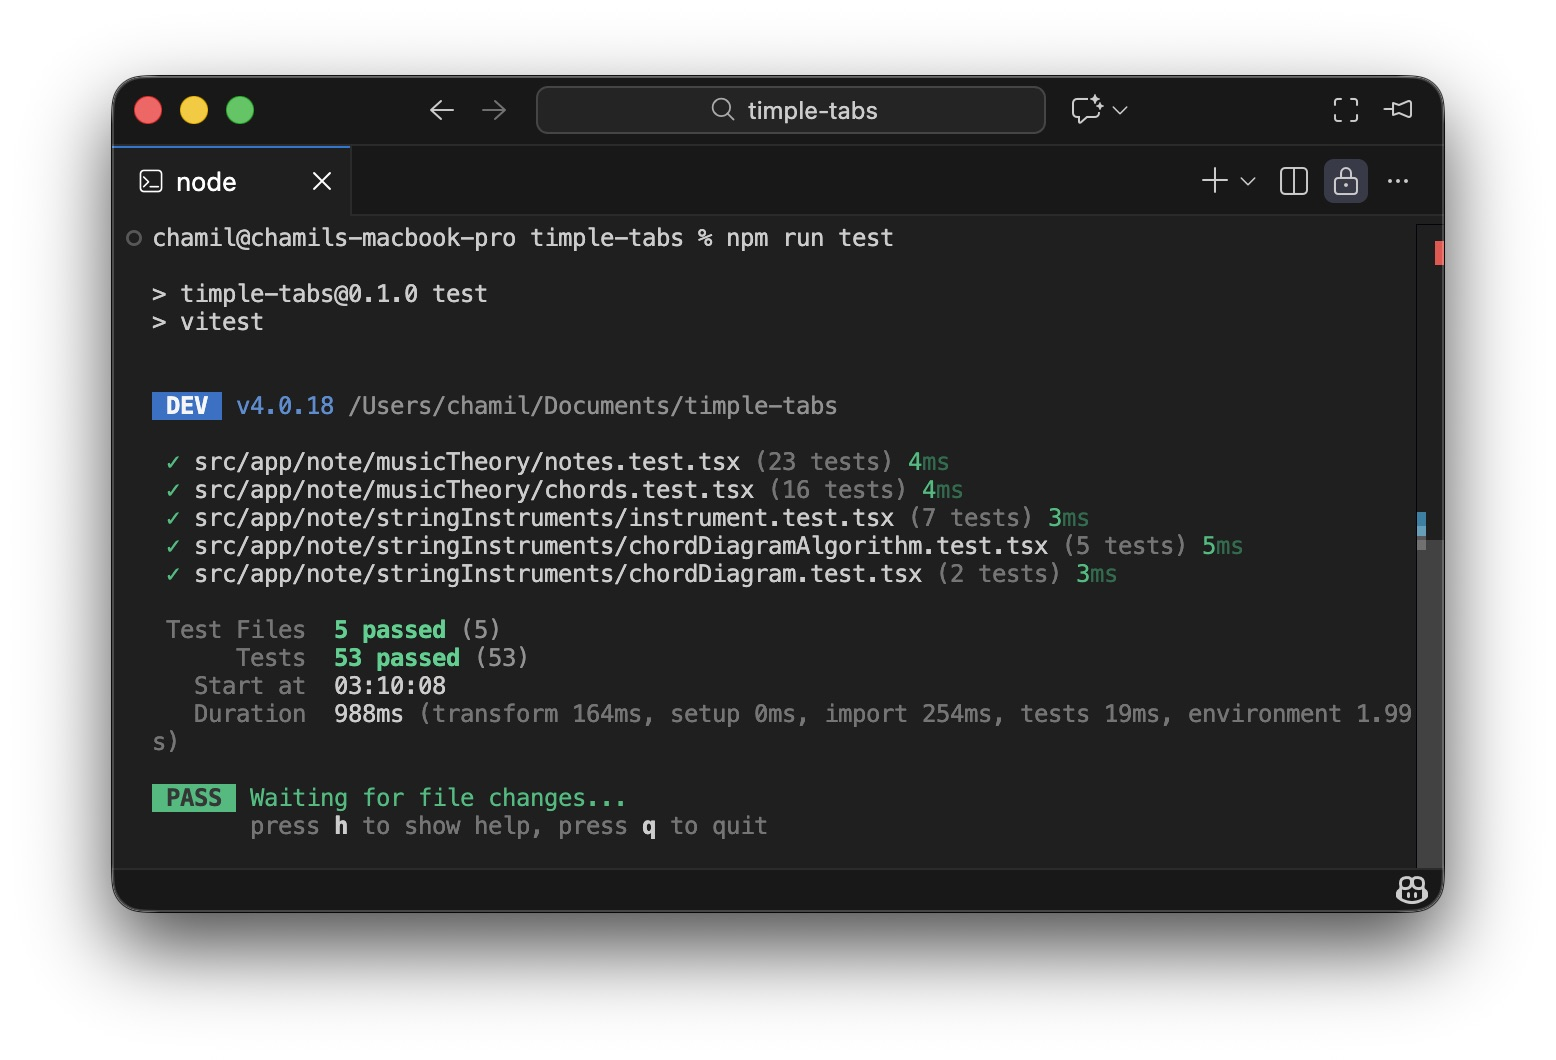
\includegraphics[width=0.8\textwidth]{Ilustraciones/desarrollo/incremento2/desarrollo/test_it2.jpeg}
    \caption{Ejecución de pruebas del incremento 2 utilizando \textit{Vitest}}\label{fig:test_it2}
\end{figure}

Por otro lado, se implementó una interfaz gráfica que imprime para un acorde dado los diagramas para timple, contra y ukelele. Se realizaron pruebas con distintos acordes \figref{fig:cmayor_it2} y \figref{fig:gmayor_it2}.

\begin{figure}[H]
    \centering
    \begin{subfigure}[t]{0.48\textwidth}
        \centering
        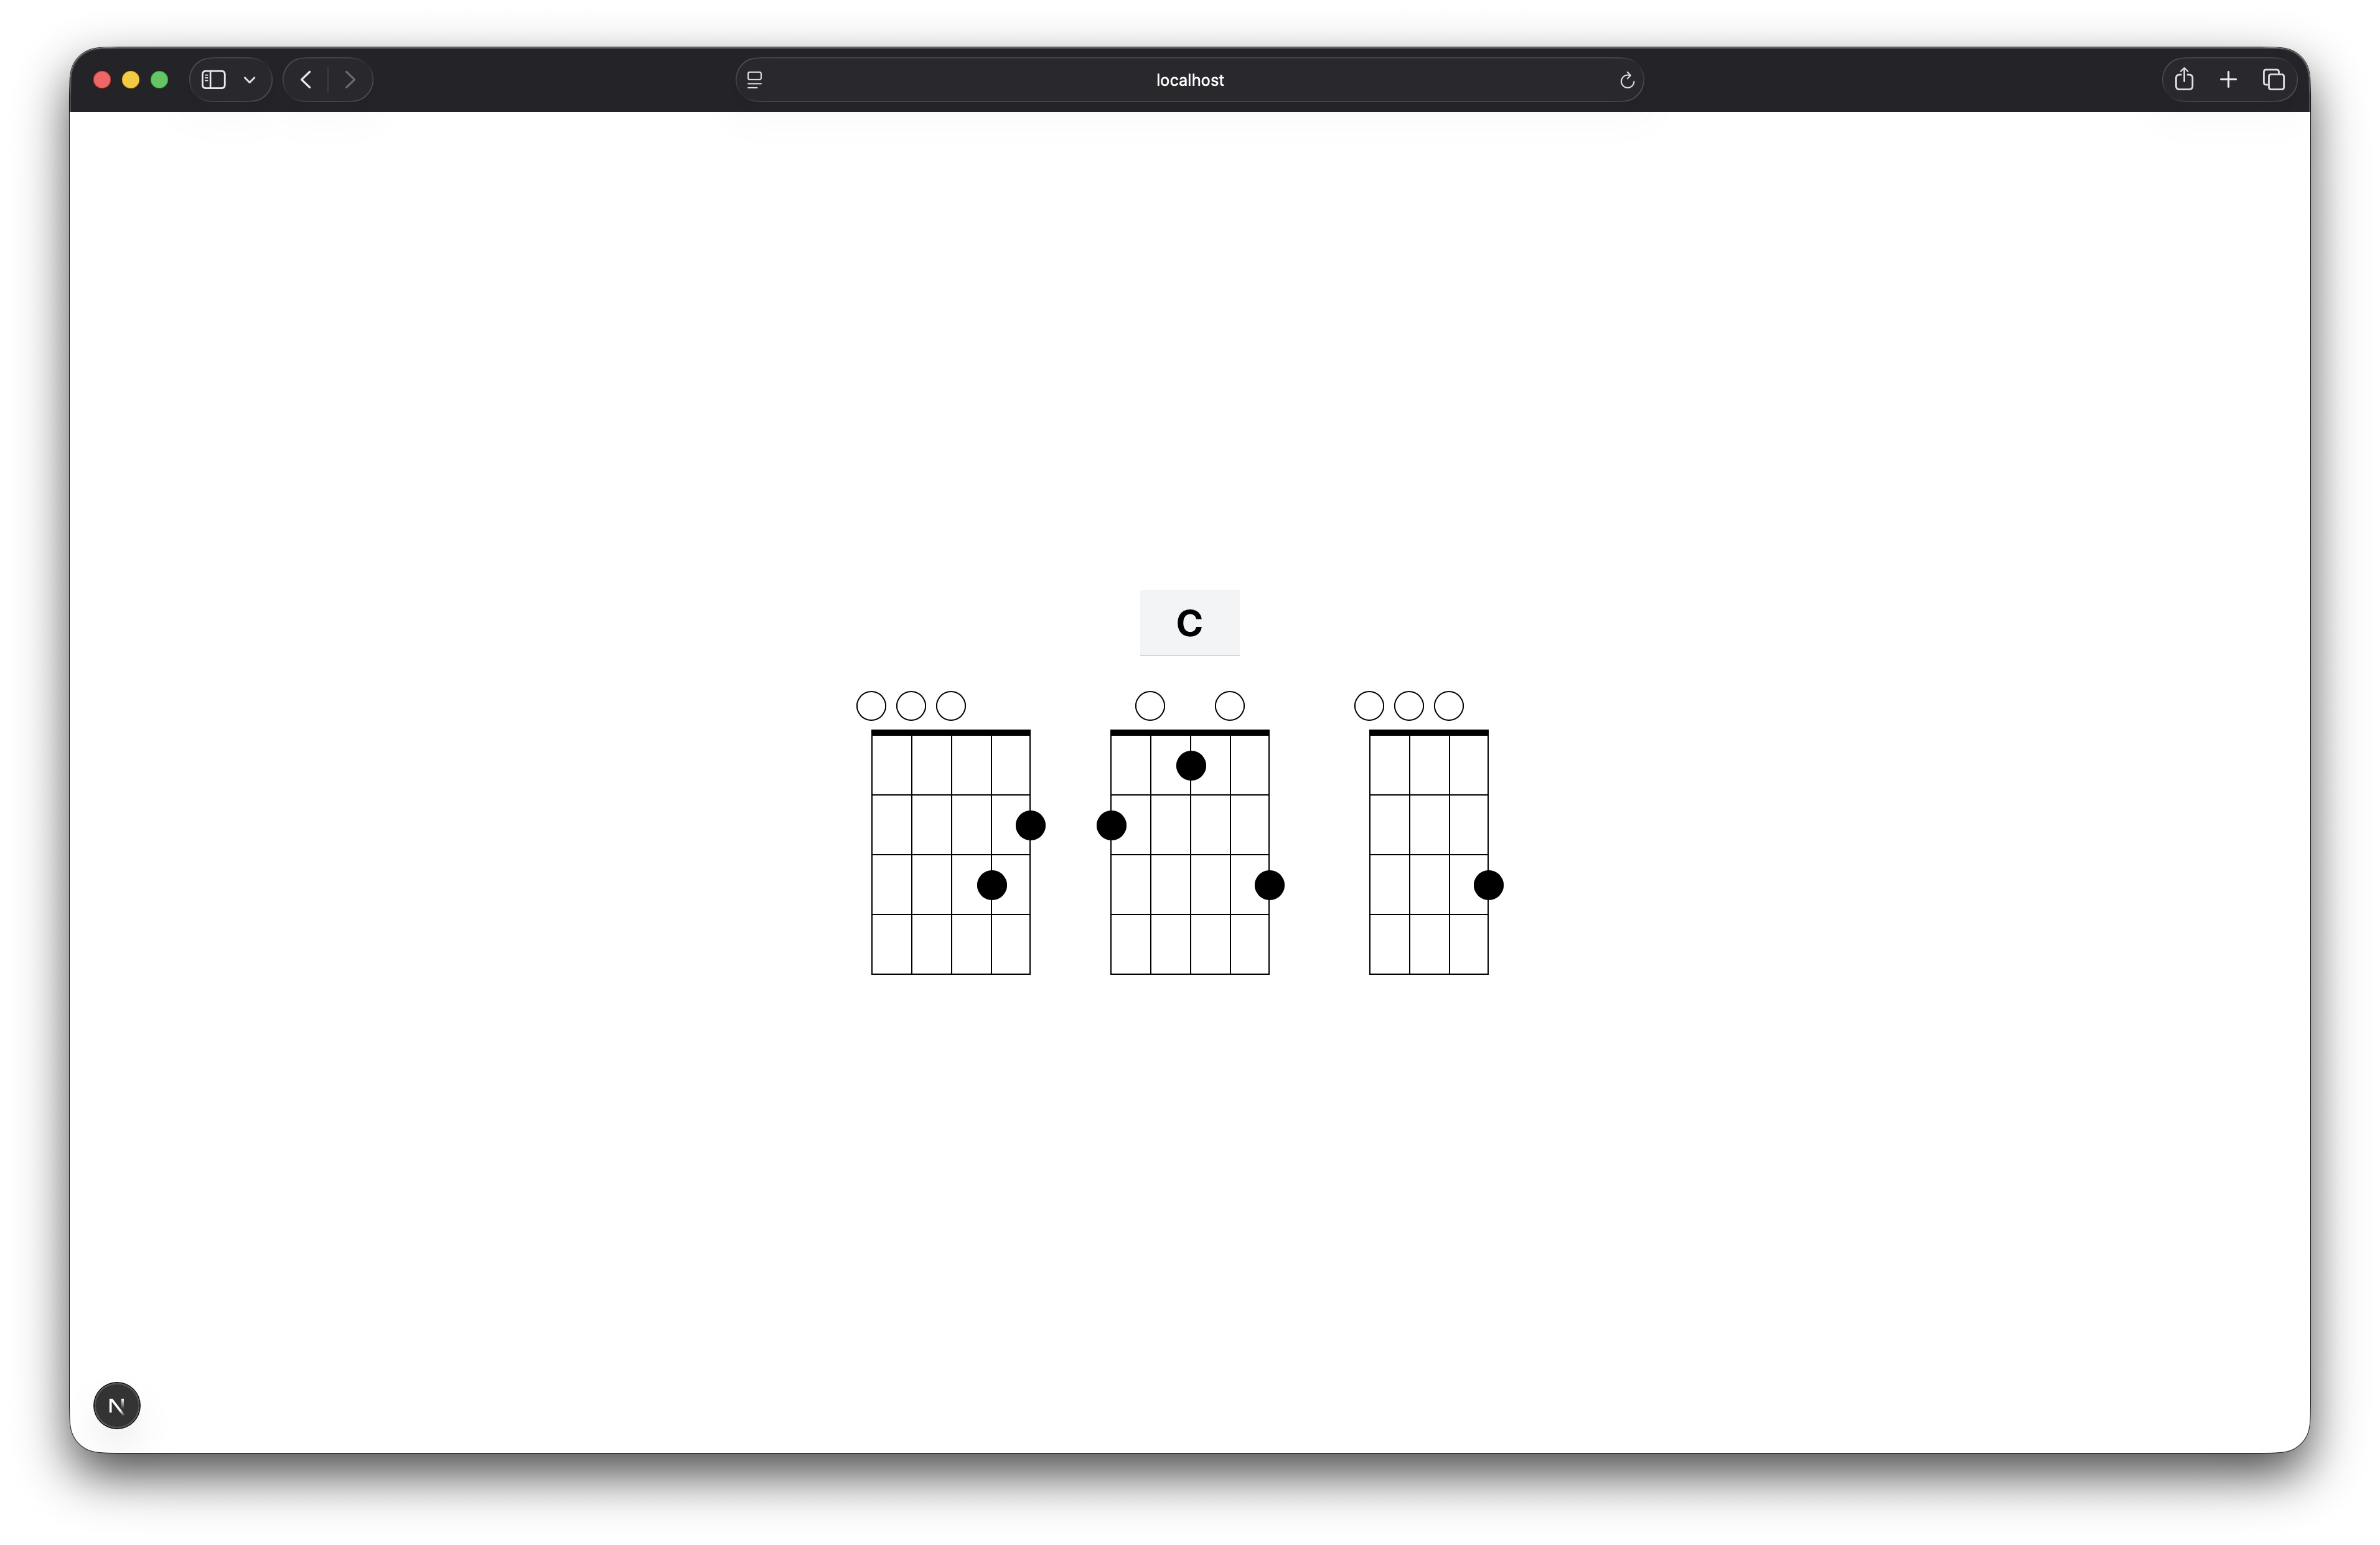
\includegraphics[width=1\textwidth]{Ilustraciones/desarrollo/incremento2/desarrollo/cmayor_it2.jpeg}
        \caption{Interfaz gráfica de prueba del incremento 2 para el acorde de \textit{C}}\label{fig:cmayor_it2}
    \end{subfigure}
    \hfill
    \begin{subfigure}[t]{0.48\textwidth}
        \centering
        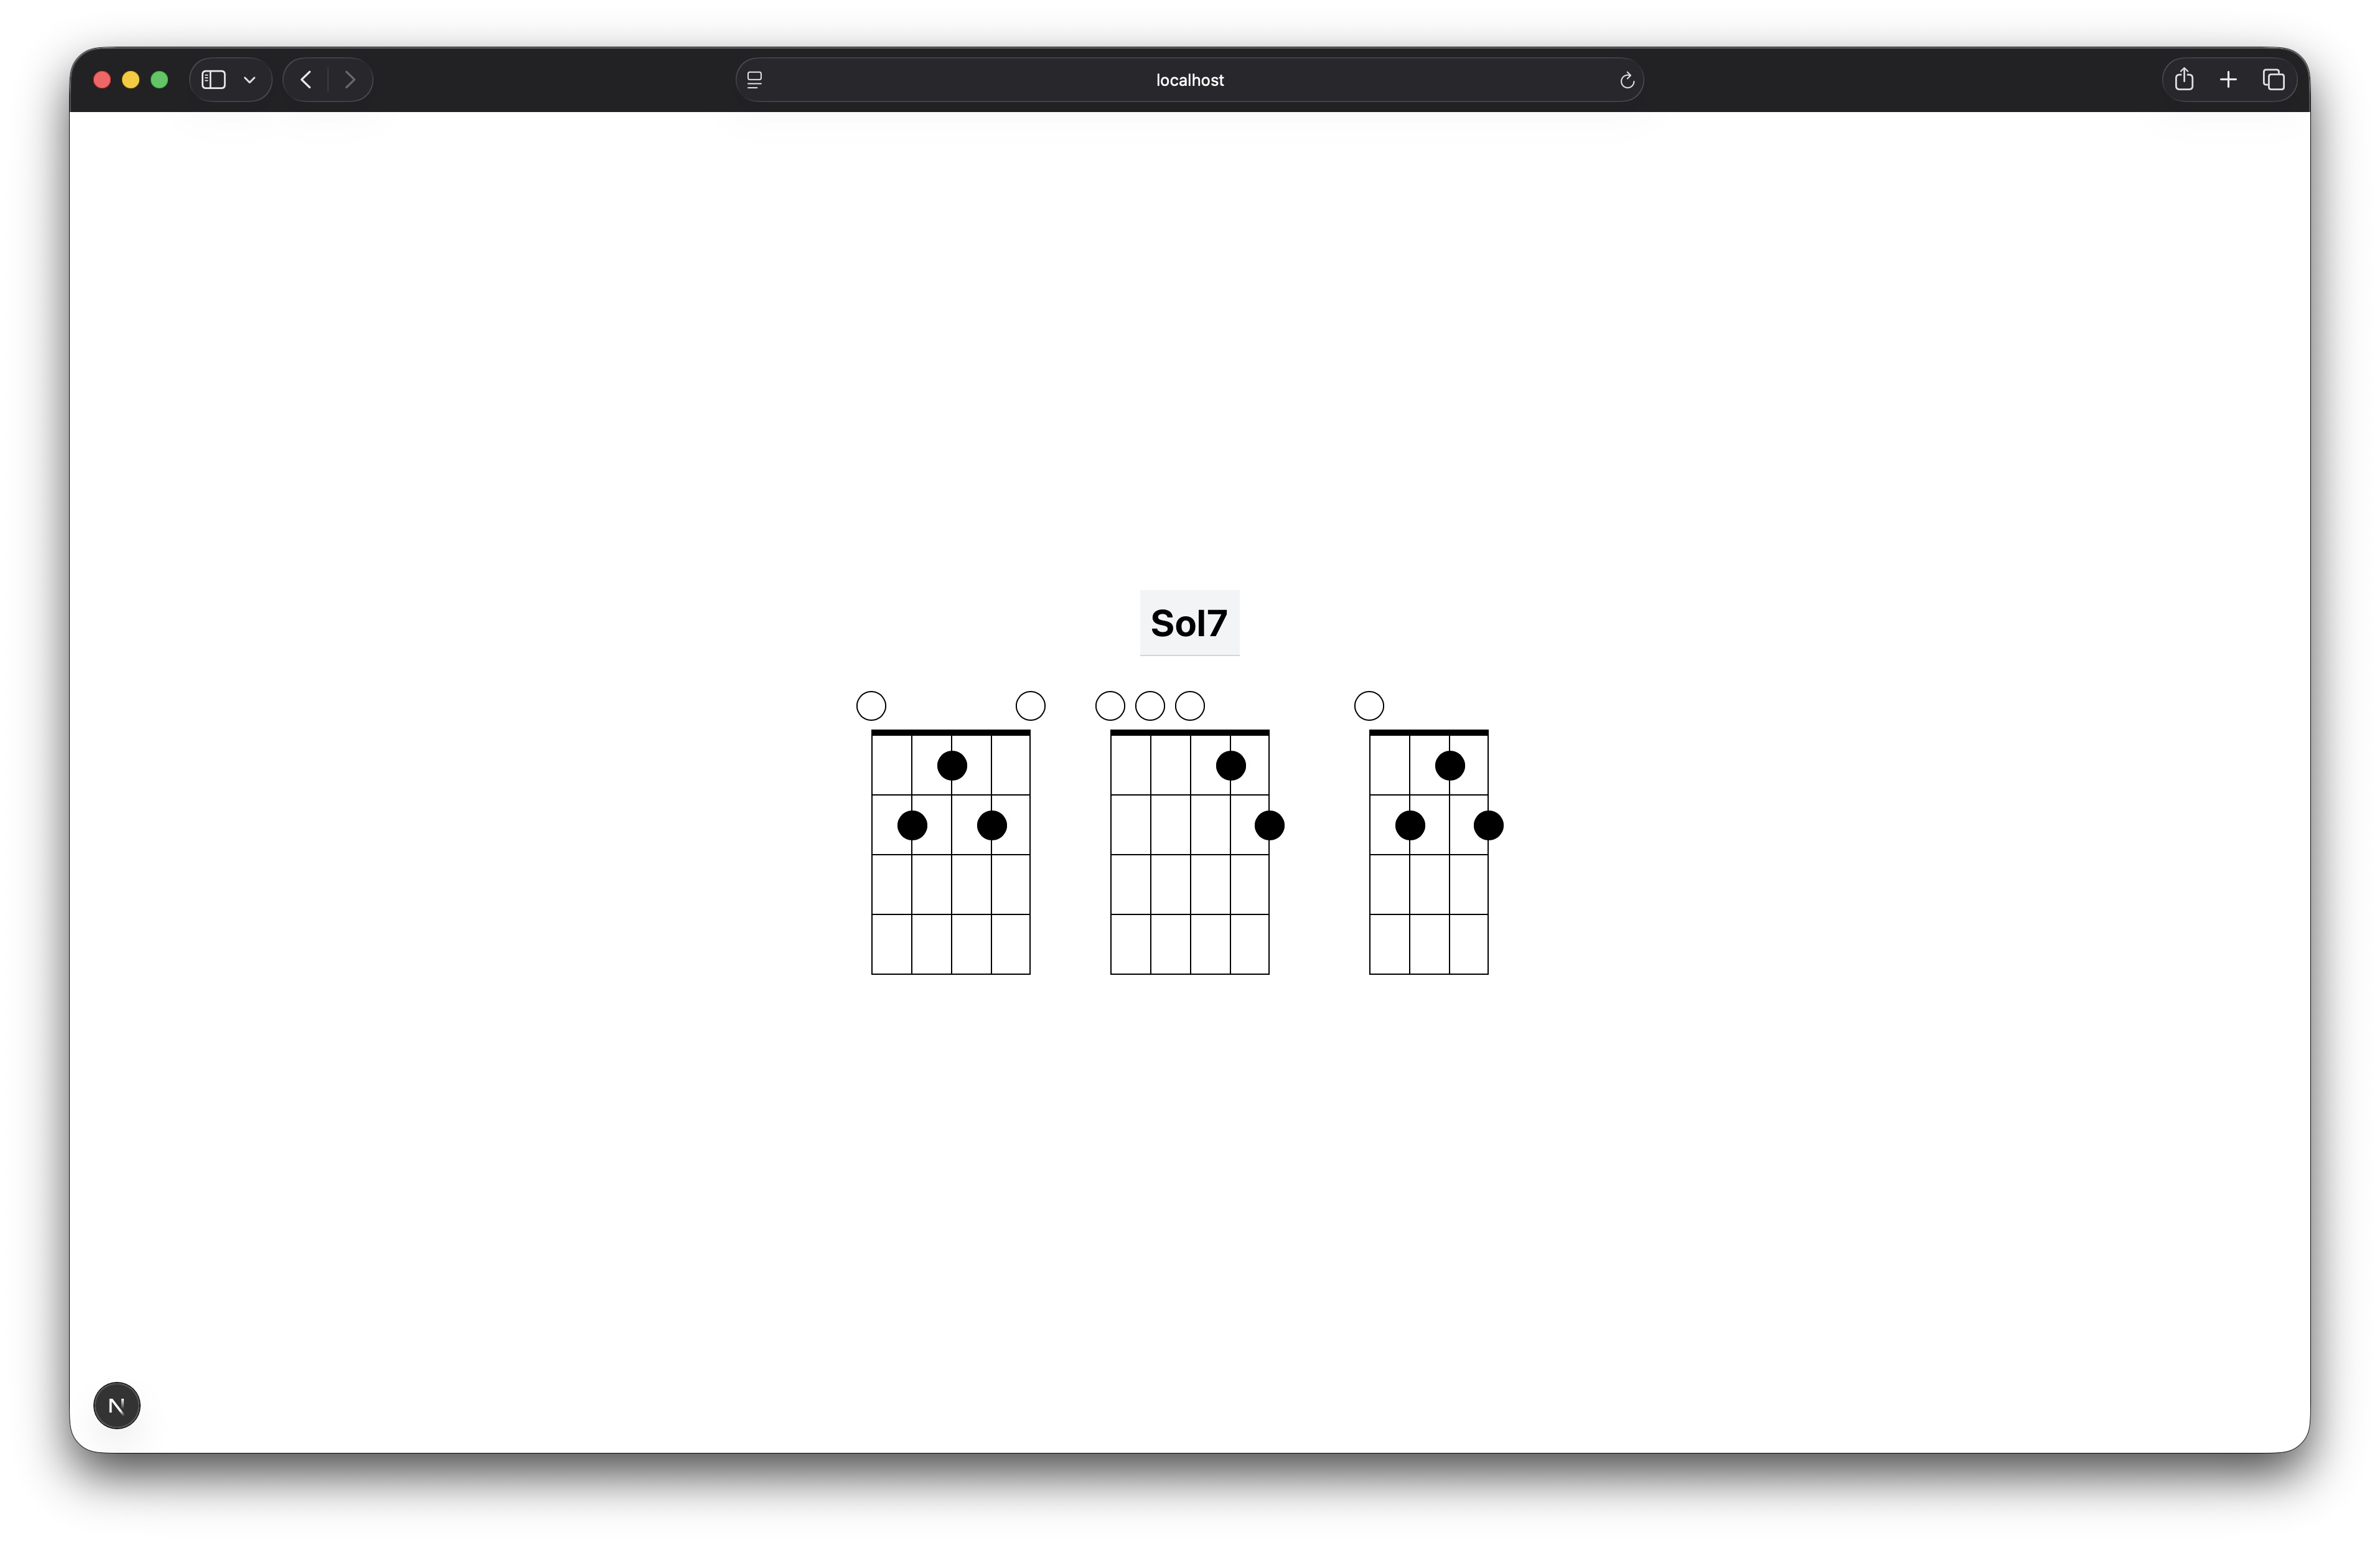
\includegraphics[width=1\textwidth]{Ilustraciones/desarrollo/incremento2/desarrollo/gmayor_it2.jpeg}
        \caption{Interfaz gráfica de prueba del incremento 2 para el acorde de \textit{Sol7}}\label{fig:gmayor_it2}
    \end{subfigure}  
    \vspace{1em}
    \caption{Diseño de diálogo de reporte}\label{fig:chord_test_it2}
\end{figure}